\documentclass[a4paper,12pt]{article}
\usepackage[utf8]{inputenc}
\usepackage[T1]{fontenc}
\usepackage{graphicx}
\usepackage{geometry}
\usepackage{tikz}
\usetikzlibrary{shapes.geometric, arrows}
\usepackage{caption}
\usepackage{subcaption}
\usepackage{float}
\usepackage[utf8]{inputenc} % UTF-8 Encoding
\usepackage[T1]{fontenc}    % Bessere Zeichendarstellung
\usepackage{array}          % Erweiterte Tabellenfunktionen
\usepackage{booktabs}       % Schönere Tabellen
\usepackage{adjustbox} % Für die automatische Skalierung


% UML tikz setup
\tikzstyle{class} = [rectangle, draw=black, text centered, text width=6cm, minimum height=1cm, rounded corners]
\tikzstyle{arrow} = [thick,->,>=stealth]

\geometry{left=2cm, right=2cm, top=2cm, bottom=2cm}

\title{Dokumentation: Klimaanlage}
\author{Chris Müller, Kilian Röper}
\date{\today}

\begin{document}
	
	\maketitle
	
	\tableofcontents
	
	\newpage
	
	\section{Einleitung}
	Dieses Dokument beschreibt eine in Simulink entwickelte Klimaanlage. Ziel ist es, alle während des Projekts entstandenen Work Products eines Worksteps innerhalb eines eigenen Kapitels zu dokumentieren. 
	
	\section{Ideenfindung und Konzeptphase}
	\subsection{Skizze der Zielanwendung aus Kundensicht}
	Die Klimaanlage dient der Regelung der Temperatur und Luftfeuchtigkeit in einem geschlossenen Raum. Die Hauptkomponenten sind:
	\begin{itemize}
		\item Ein Sensor zur Messung der aktuellen Innen- und Außentemperatur.
		\item Ein Steuergerät zur Verarbeitung der Sensordaten und Berechnung der Steuerbefehle.
		\item Aktoren wie ein Heiz-/Kühlelement.
		\item Ein Benutzerinterface zur Eingabe von Sollwerten (gewünschte Temperatur).\\
	\end{itemize}
	
	Abbildung \ref{fig:zielanwendung} zeigt eine schematische Darstellung der Klimaanlage.
	
	\begin{figure}[h!]
		\centering
		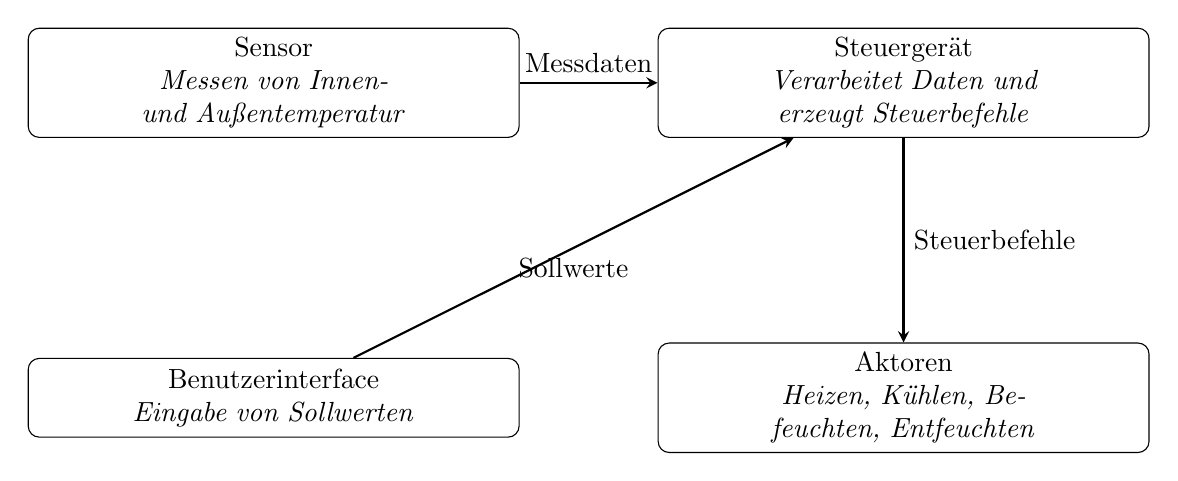
\begin{tikzpicture}[node distance=4cm]
			% Nodes
			\node (sensor) [class] {Sensor \\ \textit{Messen von Innen- und Außentemperatur}};
			\node (controller) [class, right of=sensor, xshift=4cm] {Steuergerät \\ \textit{Verarbeitet Daten und erzeugt Steuerbefehle}};
			\node (actuators) [class, below of=controller] {Aktoren \\ \textit{Heizen, Kühlen, Befeuchten, Entfeuchten}};
			\node (user) [class, left of=actuators, xshift=-4cm] {Benutzerinterface \\ \textit{Eingabe von Sollwerten}};
			
			% Arrows
			\draw [arrow] (sensor) -- (controller) node[midway, above] {Messdaten};
			\draw [arrow] (controller) -- (actuators) node[midway, right] {Steuerbefehle};
			\draw [arrow] (user) -- (controller) node[midway, below] {Sollwerte};
		\end{tikzpicture}
		\caption{Schematische Darstellung der Klimaanlage}
		\label{fig:zielanwendung}
	\end{figure}
	
	\newpage
	\subsection{Anforderungen aus Kundensicht}
	\begin{table}[h!]
		\centering
		\renewcommand{\arraystretch}{1.5} % Erhöht Zeilenabstand
		\begin{tabular}{|p{1.5cm}|p{13cm}|}
			\hline
			\textbf{Nr.} & \textbf{Anforderung} \\
			\hline
			1 & Die Klimaanlage muss in der Lage sein, die Innenraumtemperatur in einem Bereich von 16°C bis 28°C zu regeln. \\
			\hline
			2 & Die Klimaanlage muss bei allen üblichen Außentemperaturen zwischen -20°C und +50°C zuverlässig funktionieren. \\
			\hline
			3 & Die Klimaanlage soll das Fahrzeug innerhalb von 5 Minuten auf eine angenehme Temperatur herunterkühlen oder aufheizen. \\
			\hline
			4 & Die Temperatur im Fahrzeuginnenraum soll konstant gehalten werden und Schwankungen von ±1°C nicht überschreiten. \\
			\hline
			5 & Die Klimaanlage soll einen Automatikmodus besitzen, der selbstständig die ideale Temperatur auf Innen- und Außentemperatur regelt. \\
			\hline
			6 & Bei einem Defekt oder einem ungewöhnlich hohen Energieverbrauch soll die Klimaanlage in einen sicheren Modus wechseln, der keine weiteren Schäden verursacht und einen Hinweis im Fahrzeugdisplay gibt. \\
			\hline
		\end{tabular}
		\caption{Zusammenfassung der Kundenanforderungen für die Klimaanlage}
		\label{tab:kundenanforderungen}
	\end{table}
	
	\section{Anforderungsanalyse}
	\subsection{Software-Anforderungen}
	\begin{table}[H]
		\centering
		\renewcommand{\arraystretch}{1.5} % Erhöht Zeilenabstand
		\begin{tabular}{|p{1.5cm}|p{13cm}|}
			\hline
			\textbf{Nr.} & \textbf{Anforderung} \\
			\hline
			1 & Die Klimaanlagensteuerung muss die Temperatur auf eine voreingestellte Zieltemperatur zwischen 16°C und 28°C regeln können. \\
			\hline
			2 & Die Software muss die Klimaanlage so steuern, dass sie die Innenraumtemperatur in maximal 5 Minuten um mindestens 10°C herunterkühlen oder aufheizen kann. \\
			\hline
			3 & Die Software muss die Innenraumtemperatur auf ±1°C der eingestellten Zieltemperatur halten. \\
			\hline
			4 & Die Klimaanlage muss basierend auf der Innenraum- und Außentemperatur selbständig die Innenraumtemperatur auf den vom Nutzer eingestellten Sollwert regeln. \\
			\hline
			5 & Die Software muss eine Fehlererkennungsfunktion implementieren, die bei Außentemperaturen ab -20°C und niedriger, sowie +50°C und höher, einen Sicherheitsmodus aktiviert. \\
			\hline
			6 & Die Software muss eine Fehlererkennungsfunktion implementieren, die bei einem Energieverbrauch größer als 5kW einen Sicherheitsmodus aktiviert. \\
			\hline
			7 & Im Sicherheitsmodus muss die Klimaanlage deaktiviert werden, bis der Energieverbrauch wieder unter 5kW und die Temperatur wieder über -20°C oder unter 50°C beträgt. \\
			\hline
			8 & Eine Meldung „Klimaanlage im Sicherheitsmodus“ muss im Fahrzeugdisplay erscheinen, wenn der Sicherheitsmodus aktiviert ist. \\
			\hline
			9 & Die Temperatur muss in 1°C Schritten zwischen 16°C und 28°C vom Nutzer am Bedienelement der Klimaanlagensteuerung eingestellt werden können. \\
			\hline
		\end{tabular}
		\caption{Zusammenfassung der Softwareanforderungen für die Klimaanlagensteuerung}
		\label{tab:softwareanforderungen}
	\end{table}
	
	\newpage
	
	\section{Software Architektur}
	\subsection{Softwarearchitektur als Simulink-Diagramm}
	\begin{figure}[h!]
		\centering
		\includegraphics[width=\textwidth]{sw_architektur.png}
		\caption{Architektur der Software}
	\end{figure}
	\subsection{Schnittstellen}
	\begin{table}[h!]
		\centering
		\renewcommand{\arraystretch}{1.5} % Zeilenhöhe anpassen
		\begin{tabular}{@{} p{3cm} p{4cm} p{3cm} p{3cm} p{4cm} @{}}
			\toprule
			\textbf{Schnittstelle} & \textbf{Zweck} & \textbf{Datentyp} & \textbf{Wertebereich} & \textbf{Weitere Informationen} \\
			\midrule
			q\_out & Heiz- und Kühlleistungswert zur Regelung der Leistungszufuhr zu den Heiz - bzw. Kühlelementen & Integer & -5000–5000 & eine Bereichsüberschreitung führt zu einem Fehler \\
			A bis G & Pin Ausgänge zum 7 Segment Display auf dem Nucleo-Board Shield & bool & 0-1 & nur boolsche Werte erlaubt \\
			select & Signal zur Whal zwischen den beiden Displays & bool & 0–1 & wird von einer Software-internen Clock angetrieben, zur Wahl zwischen den beiden Displays \\
			\bottomrule
		\end{tabular}
		\caption{Liste der Schnittstellen}
		\label{tab:schnittstellen}
	\end{table}
	
	\newpage
	
	\section{Software Design}
	
	\subsection{Softwaredesign als Simulink Modell}
	
	
	
	\begin{figure}[h!]
		\centering
		\includegraphics[width=\textwidth]{user_interface.png}
		\caption{User Interface der Software}
	\end{figure}
	\newpage
	\begin{figure}[h!]
		\centering
		\includegraphics[width=\textwidth]{segment_display.png}
		\caption{7-Segment-Display Ansteuerung zum Shield der Software}
	\end{figure}
	\begin{figure}[h!]
		\centering
		\includegraphics[width=\textwidth]{input_system.png}
		\caption{Eingabe System der Software}
	\end{figure}
	\newpage
	\begin{figure}[h!]
		\centering
		\includegraphics[width=\textwidth]{regler.png}
		\caption{Leistungsregler der Software zur Temperaturregelung}
	\end{figure}
	\begin{figure}[h!]
		\centering
		\includegraphics[width=\textwidth]{security_block.png}
		\caption{Sicherheitsblock der Software zur Sicherstellung entsprechender Leistung und Temperatur}
	\end{figure}
	
	\newpage
	
	\subsection{Funktionalität der einzelnen Units}
	\begin{table}[h!]
		\centering
		\renewcommand{\arraystretch}{1.5} % Zeilenhöhe anpassen
		\adjustbox{max width=\textwidth}{ % Tabelle auf Seitenbreite skalieren
			\begin{tabular}{@{} p{3cm} p{5cm} p{7cm} @{}}
				\toprule
				\textbf{Softwareunit} & \textbf{Zweck} & \textbf{Umsetzung} \\
				\midrule
				User Interface (Abb.3)& Eingabe aller vom Nutzer bestimmten Eingaben, wie der on-off button oder die Zieltemperatur &  Implementierung zweier Module. Eines soll den button input verarbeiten und der das andere soll die Temperatureingabe auf das 7 Segment Display mappen\\
				7-Segment-Display (Abb. 4)& mappen der Temperatureingabe auf die 7 Steuerpins für das Nucleo Board & Implementierung einer Matlbab-Internen Funktion die die Aufgabe des Mappens übernimmt\\
				Eingabe System (Abb. 5)& Verarbeitung des Buttons und der Nutzertemperatur &  Der Button State muss gespeichert werden. Dafür muss ein Latch verwendet werden. Wird eine Eingabe vom Board für die Temperatur genutzt (ADC), dann wird über den ADC Converter der Wert in einen entsprechenden Temperaturwert zwischen 16-28°C umgerechnet \\
				Leistungsregler (Abb. 6)& Regelung der Leistung zur Temperatureinstellung & Implementierung mit einem PI Regler der Innenraumtemperatur entsprechend der vom Nutzer gewählten Temperatur einstellt \\
				Sicherheitsblock (Abb. 7)& Abschalten der Reglung wenn Temperatur oder Leistungswerte über- oder unterschritten werden & Implementierung mit einer if-else Abfrage. Die derzeitige Temperatur und Leistung sind die Eingaben. \\
				\bottomrule
			\end{tabular}
		}
		\caption{Liste der Schnittstellen}
		\label{tab:schnittstellen}
	\end{table}
	
	\newpage
	
	\subsection{Liste der Schnittstellen}
	\begin{table}[h!]
		\centering
		\renewcommand{\arraystretch}{1.5} % Zeilenhöhe anpassen
		\begin{tabular}{@{} p{3cm} p{4cm} p{3cm} p{3cm} p{4cm} @{}}
			\toprule
			\textbf{Schnittstelle} & \textbf{Zweck} & \textbf{Datentyp} & \textbf{Wertebereich} & \textbf{Weitere Informationen} \\
			\midrule
			current \_temperatur & Rückführung der Temperatur zur kontinuierlichen Regelung & double & -20 -- 50 & dieser Bereich darf nicht überschritten werden \\
			on-off-button & Nutzereingabe zum Ein- oder Ausschalten der Regelungsanlage & bool & 0-1 & nur boolsche Werte erlaubt \\
			q\_out & Heiz- und Kühlleistungswert zur Regelung der Leistungszufuhr zu den Heiz - bzw. Kühlelementen & Integer & -5000-5000 & eine Bereichsüberschreitung führt zu einem Fehler \\
			A bis G & Pin Ausgänge zum 7 Segment Display auf dem Nucleo-Board Shield & bool & 0-1 & nur boolsche Werte erlaubt \\
			select & Signal zur Whal zwischen den beiden Displays & bool & 0–1 & wird von einer Software-internen Clock angetrieben, zur Wahl zwischen den beiden Displays \\
			\bottomrule
		\end{tabular}
		\caption{Liste der Schnittstellen}
		\label{tab:schnittstellen}
	\end{table}
	
	\newpage
	
	\section{Implementation}
	\subsection{Model Guidelines}
	Um die einzelnen Einheiten lesbarer und übersichtlicher zu gestalten, wurden folgende Modellrichtlinien berücksichtigt:
	
	\subsubsection{Blockfarben}
	Für unser Modell wurden t, die folgenden Blockfarben verwendet:
	
	\begin{table}[h!]
		\centering
		\begin{tabular}{|c|l|}
			\hline
			\textbf{Farbe} & \textbf{Funktion} \\ \hline
			Rot & Inports \\ \hline
			Grün & Outports \\ \hline
			Orange & Konstanten und Gains \\ \hline
			Hellblau & MATLAB-eigene Funktionsblöcke \\ \hline
		\end{tabular}
		\caption{Farbliche Zuordnung der Blockfunktionen}
	\end{table}
	
	\subsubsection{Millersche Zahl}
	Die Units enthalten jeweils die 5 $\pm$ 2 Komponenten...
	
	\subsubsection{Einordnung in Hierarchien und Wiederverwendbarkeit}
	Wie bereits in den Abschnitten Softwaredesign und Architektur dargestellt, unterteilen sich unsere Komponenten in einzelne Units, welche die jeweilige Implementierung beinhalten. Ziel ist es, die Funktionen einzelner Codeabschnitte so zu kapseln, dass diese ohne gro\ss{}en Aufwand wiederverwendbar sind. Hierbei können einzelne Units ebenfalls wieder Units enthalten. 
	
	\subsubsection{Signalfluss}
	Der Signalfluss verläuft typischerweise von links nach rechts, nur die Rückführung der Signale erfolgt in umgekehrter Richtung. In diesem Modell gibt es nur einen Fall, nämlich die Rückführung der Regelstreckenausgangsgröße (thermical vehical body).
	
	\subsection{Beispiel zur Implemeniterung}
	Die Abbildung \ref{fig:Ersters_Softtwaremodell} zeigt eine frühe Implementierung unseres Models die alles versucht testweise eine ienem Subsystem zu implemeniteren. 
%	\begin{figure} [h!]
%		\centering
%		\includegraphics[width=0.7\linewidth]{Erstes_Softwaremodell.png}
%		\caption{Ersters Softtwaremodell}
%		\label{fig:Ersters_Softtwaremodell}
%	\end{figure}
	
	Darunter sind folgede Kompnetne
	
	\begin{table}
		\centering
		\begin{tabular}{|c|l|} \hline 
			\textbf{Kompnente}& \textbf{Änderung}\\ \hline 
			7 Segmentanzeige& Nun in einem eigen en Subsystem mit den anderen Komponenten des User-Interfaces\\ \hline 
			Der Regler&  In einem eigenen subsystem\\ \hline 
			Die Regelstrecke& Auserhalb des blocks zur Code Generation\\ \hline
		\end{tabular}
		\caption{Caption}
		\label{tab:my_label}
	\end{table}
	
	Die folgende Abbildung zeigt wie die Modell Guideliens angewendet wurden sind.
%	begin{figure}[h!]
%	\centering
%	\includegraphics[width=\textwidth]{sw_architektur.png}
%	\caption{Architektur der Software}
%	\end{figure}

\begin{figure}[h!]
	\centering
	\includegraphics[width=\textwidth]{input_system.png}
	\caption{Eingabe System der Software}
\end{figure}











\section{Implementation Review}
\subsection{Review}
\subsection{vorher nachher Vergleich der Implementierung}

\newpage

\section{Software Unit Tests}
\subsection{Testdokumentation}
Zum Ausführen der Unit-Tests muss zuerst das init-Skript ausgeführt werden, um alle Variablen aus "params/ac\_params.m" im Workspace zu speichern. Danach kann in "Klimaanlage/tests/unittest" das "run\_unit\_tests.m" Skript ausgeführt werden, mit dem die funktionalen und b2b tests gestartet und geplottet werden. 
\\
Andernfalls kann das "run\_all\_tests.m" Skript ausgeführt werden wodurch alle Tests gestartet werden aber auch die Unit-Tests.

\subsection{Testergebnisse B2B-Test}  
\begin{figure}[h!]
	\centering
	\includegraphics[width=\textwidth]{b2b_test.png}
	\caption{Ergebnis des b2b-Tests}
\end{figure}
Der B2B-Test zeigt, dass die Software Komponenten (generiert aus dem Regler) sich genauso verhält wie das Simulink Model. "Power\_cool\_heat" und "Power\_cool\_heat\_SIL" verhalten sich im Plot genau gleich. Das Ergebnis ist außerdem mit einem grünen OK nach erfolgreicher Verifizierung am oberen Rand angezeigt. 

\newpage

\subsection{Testergebnisse Funktionstest}
\begin{figure}[h!]
	\centering
	\includegraphics[width=\textwidth]{fct_test.png}
	\caption{Ergebnis des funktionalen Tests}
\end{figure}
Der funktionale Test zeigt, dass sich die Software Komponente (generiert aus dem Regler) funktional so verhält wie sie sollte. Es wurde geprüft ob eine entsprechende Heiz oder Kühlleistung gelierfert wird zum Erreichen des Temperaturziels. 25°C soll gehalten werden. Bei einer Temperatur von 50°C wird ein neagtiver Wert (kühlen) und bei einer Temperatur von -20°C einer positiver Wert (Heizen) abgegeben. Bei 25°C Außentemperatur fällt keine Leistung ab, da das Ziel bereits erreicht ist. Das Ergebnis ist außerdem mit einem grünen OK nach erfolgreicher Verifizierung am oberen Rand angezeigt. 
\newpage

\section{Software Integration und Integrationstests}
\subsection{Simulink-Modell der integrierten Software}
\begin{figure}[h!]
	\centering
	\includegraphics[width=\textwidth]{sw_integration.png}
	\caption{Integrierte Software in Simulink}
\end{figure}
\subsection{Testdokumentation}
Zum Ausführen der Integrations-Tests muss zuerst das init-Skript ausgeführt werden, um alle Variablen aus "params/ac\_params.m" im Workspace zu speichern. Danach kann in "Klimaanlage/tests/integration\_test" das "run\_integration\_tests.m" Skript ausgeführt werden, mit dem die Integrationstests gestartet und geplottet werden. 
\\
Andernfalls kann das "run\_all\_tests.m" Skript ausgeführt werden wodurch alle Tests gestartet werden aber auch die Integrations-Tests.

\newpage

\subsection{Testergebnisse}
\begin{figure}[h!]
	\centering
	\includegraphics[width=\textwidth]{integration_test.png}
	\caption{Ergebnis des Integrationstests}
\end{figure}
Der Integrationstest zeigt, dass das gesamte Software Model erfolgreich ausgeführt werden kann. Hier ist bereits zu sehen, dass sich die Temperatur gehalten wird, wenn der button ausgeschalten ist. Es wird keine Leistung mehr abgegben und die Temperatur fällt nur leicht ab, weil sie von der Außentmeperatur beeinflusst wird. 

\newpage

\section{Softwaretests}
\subsection{Testdokumentation}
Zum Ausführen der Software-Tests muss zuerst das init-Skript ausgeführt werden, um alle Variablen aus "params/ac\_params.m" im Workspace zu speichern. Danach kann in "Klimaanlage/tests/qualification\_tests/" das "run\_qualification\_tests.m" Skript ausgeführt werden, mit dem die Software Tests gestartet und geplottet werden. 
\\
Andernfalls kann das "run\_all\_tests.m" Skript ausgeführt werden wodurch alle Tests gestartet werden aber auch die Software-Tests.
\subsection{Testergebnisse Qualification Test 1}
\begin{figure}[h!]
	\centering
	\includegraphics[width=\textwidth]{qualification_test_01.png}
	\caption{Ergebnis des ersten Qualification Tests}
\end{figure}
Mit den Qualification Tests wurde gezeigt, dass die generierte Software funktional so funktioniert, wie sie in den Requirements ausgelegt wurde. Der erste Test überprüt grundsätzlich, ob die vom Nutzer eingestellte Zieltemperatur erreicht wird. Dies war erfolgreich und wird mit einem einem grünen OK am oberen Rand signalisiert. Explizit wurden die Werte 28°C und 10°C verifiziert. 

\newpage

\subsection{Testergebnisse Qualification Test 2}
\begin{figure}[h!]
	\centering
	\includegraphics[width=\textwidth]{qualification_test_02.png}
	\caption{Ergebnis des zweiten Qualification Tests}
\end{figure}
Der zweite Qualification Test überprüft die funktionalität des on-off Buttons. Wenn dieser off ist, dann soll die Temperatur nicht geregelt werden, auch wenn eine Solltemperatur vom Nutzer anliegt. Dies war erfolgreich und wird mit einem grünen OK am oberen Rand signalisiert. Die Temperatur wird bei 16°C noch eine Weile gehalten, bevor die vom Nutzer eingestellten 25 angesteuert werden sobald der Button auf on gesetzt ist. 


\end{document}
